\documentclass{standalone}
\usepackage{tikz}
\usetikzlibrary{patterns, positioning}
\usetikzlibrary{shapes.misc}
\usepackage[outline]{contour}
\contourlength{1.5pt} 
\usepackage[sfdefault]{ClearSans} %% option 'sfdefault' activates Clear Sans as the default text font
\usepackage[T1]{fontenc}

\begin{document}
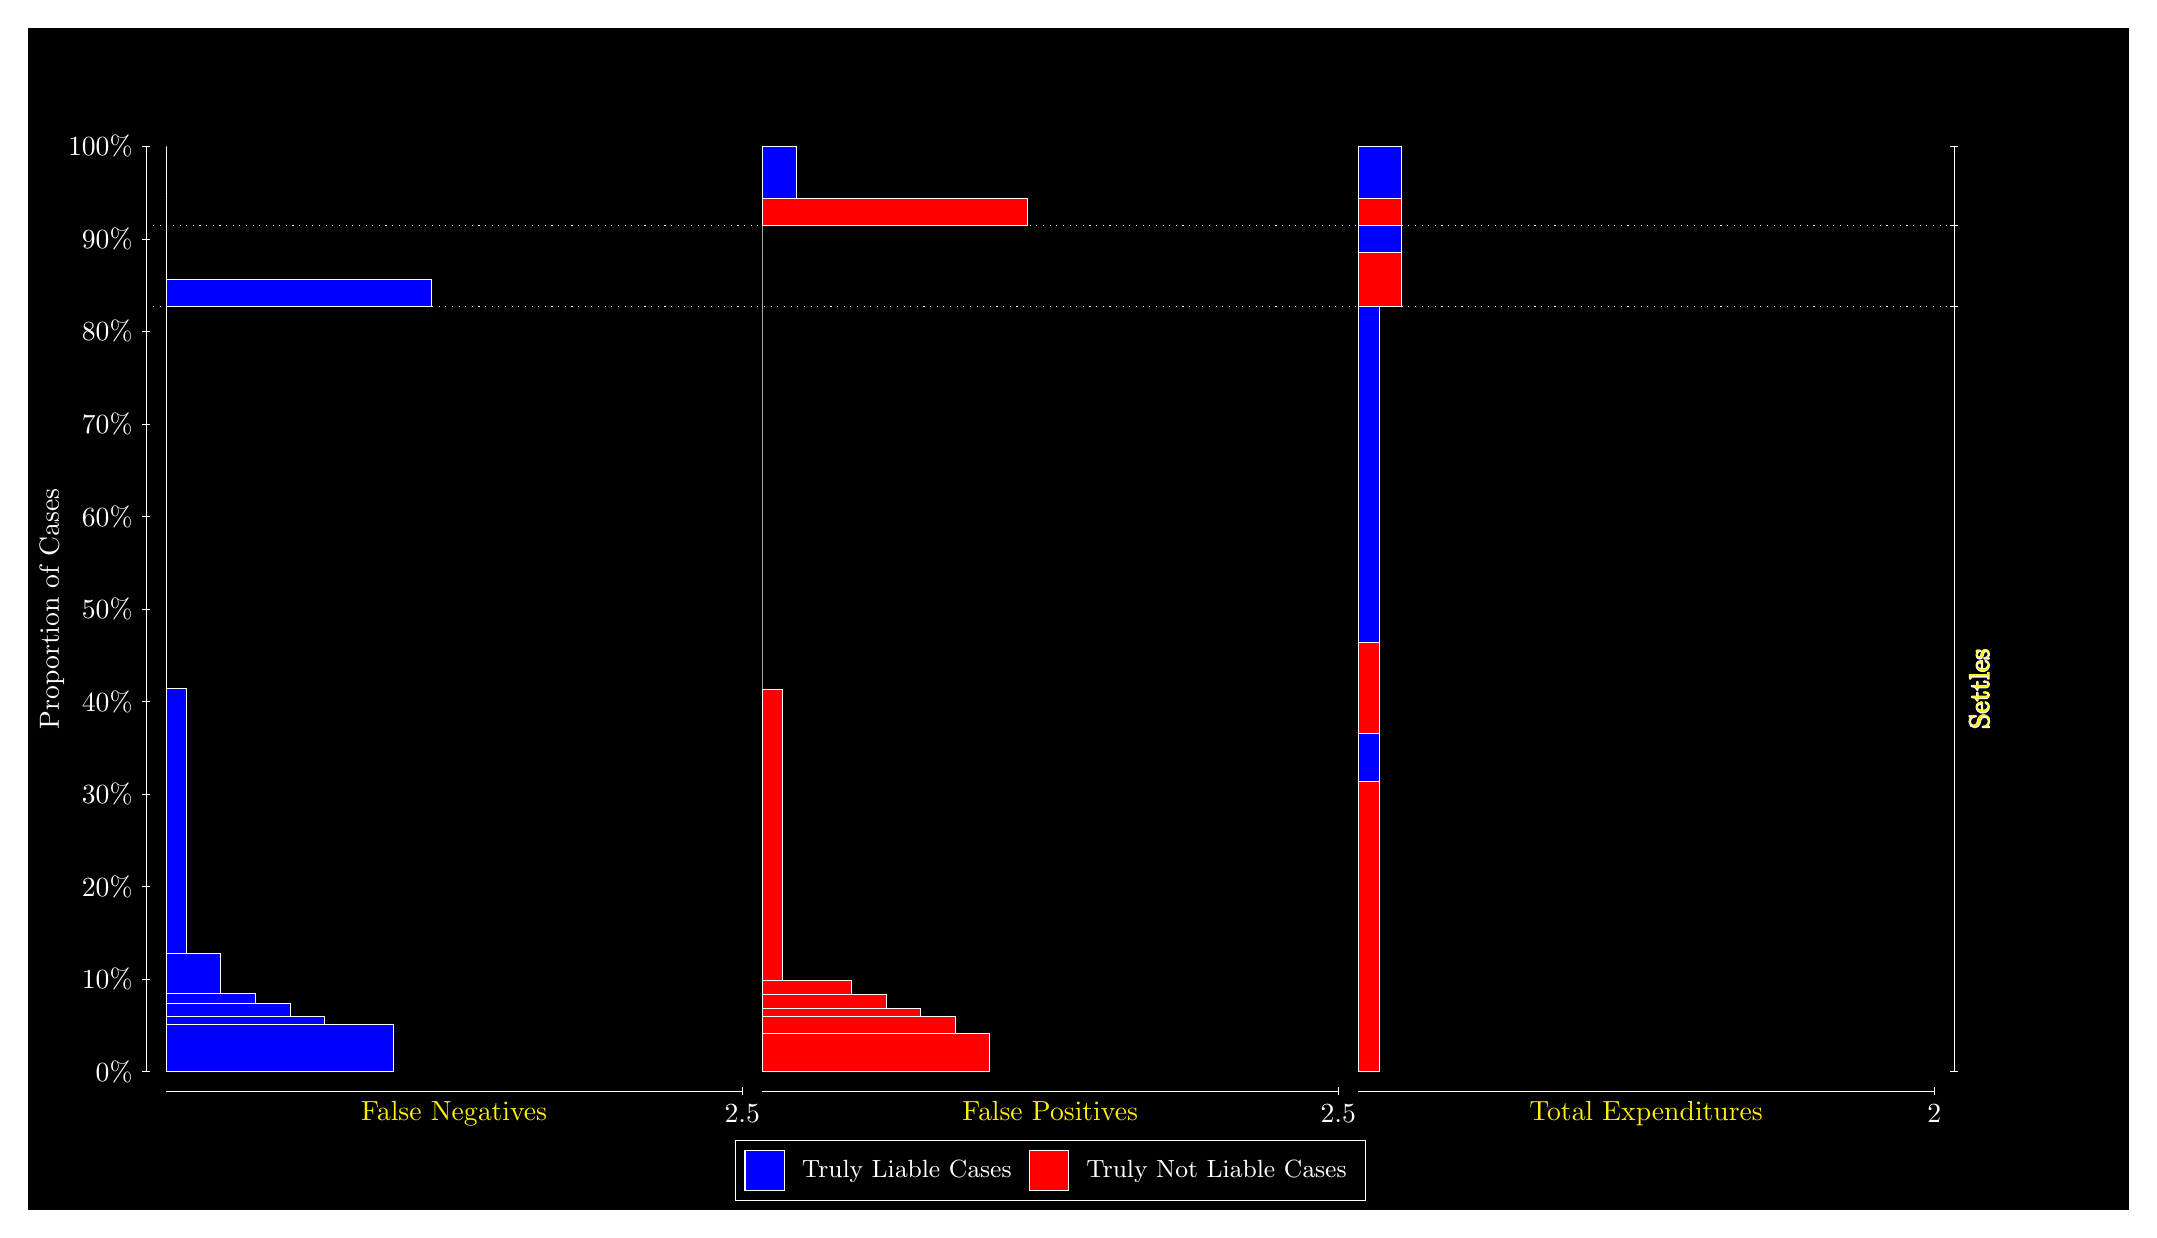
\begin{tikzpicture}
\draw[fill=black] (0,0) rectangle (26.667,15);
\draw[white, very thin] (1.5,1.75) -- (1.5,13.5);
\node[rotate=90, text=white, anchor=center] at (0.3, 7.625) {Proportion of Cases};
\draw[white, very thin] (1.45,1.75) -- (1.55,1.75);
\node[text=white, anchor=east] at (1.45, 1.75) {0\%};
\draw[white, very thin] (1.45,2.925) -- (1.55,2.925);
\node[text=white, anchor=east] at (1.45, 2.925) {10\%};
\draw[white, very thin] (1.45,4.1) -- (1.55,4.1);
\node[text=white, anchor=east] at (1.45, 4.1) {20\%};
\draw[white, very thin] (1.45,5.275) -- (1.55,5.275);
\node[text=white, anchor=east] at (1.45, 5.275) {30\%};
\draw[white, very thin] (1.45,6.45) -- (1.55,6.45);
\node[text=white, anchor=east] at (1.45, 6.45) {40\%};
\draw[white, very thin] (1.45,7.625) -- (1.55,7.625);
\node[text=white, anchor=east] at (1.45, 7.625) {50\%};
\draw[white, very thin] (1.45,8.8) -- (1.55,8.8);
\node[text=white, anchor=east] at (1.45, 8.8) {60\%};
\draw[white, very thin] (1.45,9.975) -- (1.55,9.975);
\node[text=white, anchor=east] at (1.45, 9.975) {70\%};
\draw[white, very thin] (1.45,11.15) -- (1.55,11.15);
\node[text=white, anchor=east] at (1.45, 11.15) {80\%};
\draw[white, very thin] (1.45,12.325) -- (1.55,12.325);
\node[text=white, anchor=east] at (1.45, 12.325) {90\%};
\draw[white, very thin] (1.45,13.5) -- (1.55,13.5);
\node[text=white, anchor=east] at (1.45, 13.5) {100\%};

\draw[white, very thin] (24.457,1.75) -- (24.457,13.5);
\draw[white, very thin] (24.407,1.75) -- (24.507,1.75);
\node[anchor=west] at (24.407, 1.75) {};
\draw[white, very thin] (24.407,11.469) -- (24.507,11.469);
\node[anchor=west] at (24.407, 11.469) {};
\draw[white, very thin] (24.407,12.498) -- (24.507,12.498);
\node[anchor=west] at (24.407, 12.498) {};
\draw[white, very thin] (24.407,13.5) -- (24.507,13.5);
\node[anchor=west] at (24.407, 13.5) {};

\draw[white, very thin, fill=blue] (1.75,1.75) rectangle (4.641,2.3497);
\draw[white, very thin, fill=blue] (1.75,2.3497) rectangle (3.7627,2.4459);
\draw[white, very thin, fill=blue] (1.75,2.4459) rectangle (3.3236,2.616);
\draw[white, very thin, fill=blue] (1.75,2.616) rectangle (2.8844,2.7463);
\draw[white, very thin, fill=blue] (1.75,2.7463) rectangle (2.4453,3.2553);
\draw[white, very thin, fill=blue] (1.75,3.2553) rectangle (2.0062,6.6185);
\draw[white, very thin, fill=red] (1.75,6.6185) rectangle (1.75,11.469);
\draw[white, very thin, fill=blue] (1.75,11.469) rectangle (5.1167,11.815);
\draw[white, very thin, fill=red] (1.75,11.815) rectangle (1.75,12.498);
\draw[white, very thin, fill=red] (1.75,12.498) rectangle (1.75,12.84);
\draw[white, very thin, fill=blue] (1.75,12.84) rectangle (1.75,13.5);
\draw[white, very thin, fill=red] (9.3189,1.75) rectangle (12.21,2.2305);
\draw[white, very thin, fill=red] (9.3189,2.2305) rectangle (11.771,2.4459);
\draw[white, very thin, fill=red] (9.3189,2.4459) rectangle (11.332,2.558);
\draw[white, very thin, fill=red] (9.3189,2.558) rectangle (10.892,2.7281);
\draw[white, very thin, fill=red] (9.3189,2.7281) rectangle (10.453,2.9096);
\draw[white, very thin, fill=red] (9.3189,2.9096) rectangle (9.575,6.6003);
\draw[white, very thin, fill=blue] (9.3189,6.6003) rectangle (9.3189,11.469);
\draw[white, very thin, fill=red] (9.3189,11.469) rectangle (9.3189,12.151);
\draw[white, very thin, fill=blue] (9.3189,12.151) rectangle (9.3189,12.498);
\draw[white, very thin, fill=red] (9.3189,12.498) rectangle (12.686,12.84);
\draw[white, very thin, fill=blue] (9.3189,12.84) rectangle (9.758,13.5);
\draw[white, very thin, fill=red] (16.888,1.75) rectangle (17.162,5.4407);
\draw[white, very thin, fill=blue] (16.888,5.4407) rectangle (17.162,6.0404);
\draw[white, very thin, fill=red] (16.888,6.0404) rectangle (17.162,7.2);
\draw[white, very thin, fill=blue] (16.888,7.2) rectangle (17.162,11.469);
\draw[white, very thin, fill=red] (16.888,11.469) rectangle (17.437,12.151);
\draw[white, very thin, fill=blue] (16.888,12.151) rectangle (17.437,12.498);
\draw[white, very thin, fill=red] (16.888,12.498) rectangle (17.437,12.84);
\draw[white, very thin, fill=blue] (16.888,12.84) rectangle (17.437,13.5);
\draw[white, dotted] (1.5,11.469) -- (24.457,11.469);
\draw[white, dotted] (1.5,12.498) -- (24.457,12.498);
\draw[white, very thin] (1.75,1.5) -- (9.0689,1.5);
\node[text=yellow, anchor=north] at (5.4094, 1.5) {False Negatives};
\draw[white, very thin] (9.0689,1.45) -- (9.0689,1.55);
\node[text=white, anchor=north] at (9.0689, 1.45) {2.5};

\draw[white, very thin] (9.3189,1.5) -- (16.638,1.5);
\node[text=yellow, anchor=north] at (12.978, 1.5) {False Positives};
\draw[white, very thin] (16.638,1.45) -- (16.638,1.55);
\node[text=white, anchor=north] at (16.638, 1.45) {2.5};

\draw[white, very thin] (16.888,1.5) -- (24.207,1.5);
\node[text=yellow, anchor=north] at (20.547, 1.5) {Total Expenditures};
\draw[white, very thin] (24.207,1.45) -- (24.207,1.55);
\node[text=white, anchor=north] at (24.207, 1.45) {2};

\node[text=yellow, centered, rotate=90] at (24.777, 6.6094) {\contour{white}{Settles}};



\draw (12.978300999999998,1.5) node[draw=none] (baseCoordinate) {};
\begin{scope}[align=center]
        \matrix[scale=0.5, draw=white, below=0.5cm of baseCoordinate, nodes={draw}, column sep=0.1cm]{
            \node[rectangle, draw, minimum width=0.5cm, minimum height=0.5cm, fill=blue] {}; &
            \node[draw=none, font=\small, text=white] (B) {Truly Liable Cases}; &
            \node[rectangle, draw, minimum width=0.5cm, minimum height=0.5cm, fill=red] {}; &
            \node[draw=none, font=\small, text=white] (B) {Truly Not Liable Cases}; \\
            };
\end{scope}

\end{tikzpicture}
\end{document}